%# -*- coding: utf-8-unix -*-
% !TEX program = xelatex
% !TEX root = ../thesis.tex
% !TEX encoding = UTF-8 Unicode
%%==================================================
%% chapter02.tex for SJTU Master Thesis
%% based on CASthesis
%% modified by wei.jianwen@gmail.com
%% Encoding: UTF-8
%%==================================================

\chapter{Modeling and Analysis}
\label{chap:modeling and analysis methods}

\section{Modeling of two layer network}
\label{sec:modeling of two layer network}

The model consists of two layers, and each layer has different dynamics. For layer A, the node change its states according to $M$ model as introduced in \cite{rocca2014}. Here, we choose $M=2$, that each node has four states $(-2, -1, +1, +2)$. For each link $(k, j)$ belong to layer A,  the dynamics are designed as follows:
\begin{itemize}
	\item Compromise : if two nodes connected with link$(k, j)$ have opposite orientations, their states become more moderate with probability $q$ :
	\begin{align}
	\mbox{if } S_k<0 \mbox{ and } S_j>0  \Rightarrow (S_k, S_j) \rightarrow (S_k^r, S_j^l) \mbox{ with } prob.q,\\
	\mbox{if } S_k>0 \mbox{ and } S_j<0  \Rightarrow (S_k, S_j) \rightarrow (S_k^l, S_j^r) \mbox{ with } prob.q.
	\end{align}
	If $S_k = \pm1$ and $S_j = \mp1$, one switches orientation at random:
	\begin{align}
	(\pm 1, \mp 1)\rightarrow \left\{\begin{matrix}
	(+1, +1) \mbox{ with } prob.q/2,
	\\(-1, -1)\mbox{ with } prob.q/2.
	\end{matrix}\right.
	\end{align}
	\item Persuasion : if two nodes connected with link$(k, j)$ have the same orientation, their states become more extreme with probability $p$ :
	\begin{align}
	\mbox{if } S_k<0 \mbox{ and } S_j<0  \Rightarrow (S_k, S_j) \rightarrow (S_k^l, S_j^l) \mbox{ with } prob.p,\\
	\mbox{if } S_k>0 \mbox{ and } S_j>0  \Rightarrow (S_k, S_j) \rightarrow (S_k^r, S_j^r) \mbox{ with } prob.p.
	\end{align}
\end{itemize}
For each external link $(k,j)$ with $k$ belong to layer A, the state of node $k$ is updated according to :
\begin{itemize}
	\item $S_k \cdot S_j < 0$ :
	\begin{align}
	\mbox{if } S_k<0 \mbox{ and } S_j>0  \Rightarrow (S_k, S_j) \rightarrow (S_k^r, S_j) \mbox{ with } prob.q,\\
	\mbox{if } S_k>0 \mbox{ and } S_j<0  \Rightarrow (S_k, S_j) \rightarrow (S_k^l, S_j) \mbox{ with } prob.q.
	\end{align}
	\item $S_k \cdot S_j > 0$ :
	\begin{align}
	\mbox{if } S_k<0 \mbox{ and } S_j<0  \Rightarrow (S_k, S_j) \rightarrow (S_k^l, S_j) \mbox{ with } prob.p,\\
	\mbox{if } S_k>0 \mbox{ and } S_j>0  \Rightarrow (S_k, S_j) \rightarrow (S_k^r, S_j) \mbox{ with } prob.p.
	\end{align}
\end{itemize}
Here, $S_k^r$ and $S_k^l$ denote the right and left neighboring states of $k$, defined as
\begin{align}
S_k^r &= \left\{\begin{matrix}
+1,\mbox{ for } S_k = -1\\
+2,\mbox{ for } S_k = +2\\ 
S_k + 1,\mbox{ otherwise }, 
\end{matrix}\right. &
S_k^l &= \left\{\begin{matrix}
-1,\mbox{ for } S_k= +1
\\ -2,\mbox{ for } S_k=-2
\\ S_k - 1,\mbox{ otherwise }.
\end{matrix}\right.
\end{align}

The sign of $S^A$ represents its opinion orientation and its absolute value $|S^A|$ measures the intensity of its opinion. So, $|S^A|=2$ represents to a positive or a negative extremist, while  $|S^A|=1$ correspond to a moderate opinion of each side. In case of internal link $(k, j)$ belong to layer A, when the nodes have the same orientation$(S_kS_j>0)$, if the states of nodes are moderate, then they become extreme$(S_k=\pm1 \rightarrow \pm2, S_j= \pm1 \rightarrow \pm2)$ with probability $p$. If they are already extreme, they remain extreme$(S_k=\pm2 \rightarrow \pm2, S_j= \pm2 \rightarrow \pm2)$. On the other hand, when the nodes have opposite orientations$(S_kS_j<0)$, if they are extreme, the states of nodes become moderate$(S_k=\pm2 \rightarrow \pm1, S_j= \pm2 \rightarrow \pm1)$ with probability $q$. If they are already moderate, they switch orientations individually$(S_k=\pm1 \rightarrow \mp1, S_j= \pm1 \rightarrow \mp1)$.  In case of interaction between node in layer A and node in layer B, node in layer A follows opinion dynamics formula, but the state of node in layer B does not change. In other words, the state of layer B affects layer A, but layer A dynamics does not affect the state of node in layer B. For example, one of the layer A node, $S_k = +2$ is connected with  $S_j = -1$ node of layer B. Here, $S_k$ will change into $S_k = +1$ with $prob.q$. But $S_j$ will not change, which indicates that the states of layer B will influence the states of layer A.

The dynamics of layer B follows the decision-making dynamics as introduced in \cite{abrams2003, vazquez2010}. The state of node i in layer B can be $+1$ and $-1$, and it updates according to

\begin{equation}
{P_B}({S_i} \to  - {S_i}) = \begin{cases}
{\left({\displaystyle\frac{{{i_i} + {e_i}}}{{{n^{ - {S_i}}}}}}\right)}{\cdot}{\left({\displaystyle\frac{{n^{-{S_i}}}}{{{i_i} + {e_i}}}} \right)^{1/v}}  ,\mbox{ if } v \ne 0\\
0,\mbox{ if } v = 0\\
0,\mbox{ if } {n^{ - {S_i}}} = 0
\end{cases},
\end{equation}

where $i_i$ is the number of internal edges and $e_i$ is the number of external edges. $n^{-S_i}$ is the number of neighbors of i with opposite state $-S_i$. $v$ represents the volatility that measures how prone a node change its state. The scale of $v$ is from $0$ to $1$. If $v \simeq 0$,  a node is unlikely to change its state. On the other hand, if $v \simeq 1$, a node is very likely to change its state. Also, this formula shows that the more the number of nodes connected with the opposite state is, the easier the nodes are to change into the opposite state.\\
\begin{figure}[!htb]
	\centering
	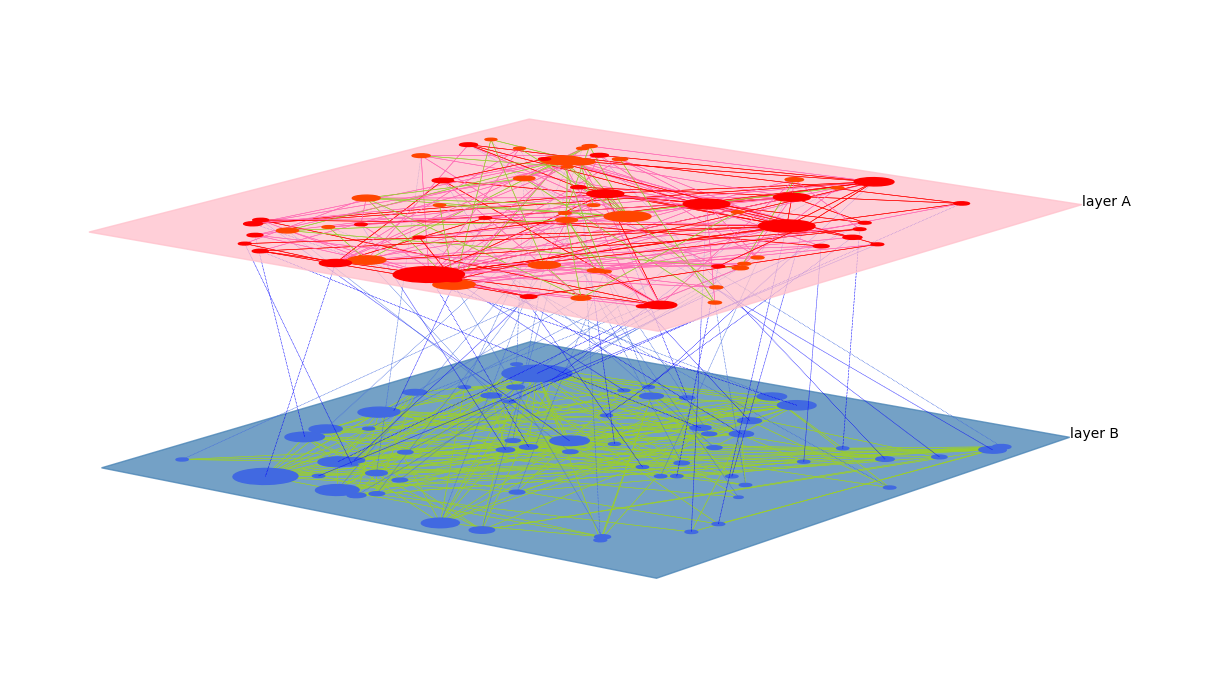
\includegraphics[width=\hsize]{FIG1.png}
	\caption{Competition of Interconnected Network}
	\label{Fig1}
\end{figure}

\section{Simulations and Analysis}
To start with a polarized competition, as the initial conditions,  nodes in layer A are all positive, and nodes in layer B are all negative as shown in Fig.~\ref{Fig1}. For nodes in layer A, it begins with the status where half of nodes are $+1$ and the others are $+2$. The initial state of nodes in layer B have only $-1$. 

There are two parameters in the dynamics of layer A. To simply represent the probability $p$ and probability $q$ together, we set $p+q=1$. So, $p$ represents the tendency of opinion such as extreme or moderate, which is scaled to be $0$ to $1$. And, the scale of $v$, in the dynamics of layer B, is also $0$ to $1$. 

To implement the interconnected dynamics, one step consists of two layers dynamics, where every node in layer A will be checked with opinion dynamics, and every node in layer B will updates its state according to the decision-making dynamics. Here, we would control dynamics orders between layers and updating rules of nodes states. With changing dynamics orders and updating rules, it would be investigated how state of network change.      

Each simulation takes $100$ steps, and $100$ simulations are considered for average results. In the following simulations, we use \textit{`Average State'(AS)} and \textit{`Consensus Index'(CI)} to measure the competition result.

\begin{equation}
AS = avg\left( {\sum\limits_i^{{K^A}} {S_i^A/4} } \right) + avg\left( {\sum\limits_i^{{K^B}} {S_i^B/2} } \right).
\end{equation}

\begin{equation}
CI = \frac{{({K_ + }^A \cdot {K_ - }^B) + ({K_ - }^A \cdot {K_ + }^B)}}{{{K^A} \cdot {K^B}}}
\end{equation}

In these formula, $S_i^A$ means the state of node \textit{i} in layer A, and $K^A$ is the number of nodes in layer A. ${K_ + }^A$ represents the number of nodes with positive state in layer A.   

With \textit{AS}, it could be verified whether the consensus happens in accordance with the change of $p$ and $v$.  If the positive consensus happens, it would be close to the value of $+1$ and if the negative consensus happens, it would be close to the value of $-1$. The values between $+1$ and $-1$ mean the states are belonging to the coexistence part.

With \textit{CI}, it could be measured how close the network state is to consensus. If the CI is close to $0$, the state is close to positive or negative consensus. If the CI is close to $1$, the state is separated coexistence where states of all nodes in layer A is opposed to states of all nodes in layer B. If the CI is close to $0.5$, the state is mixed coexistence where each layer has both positive and negative states of nodes.    

\begin{figure*}[!htb]
	\centering
	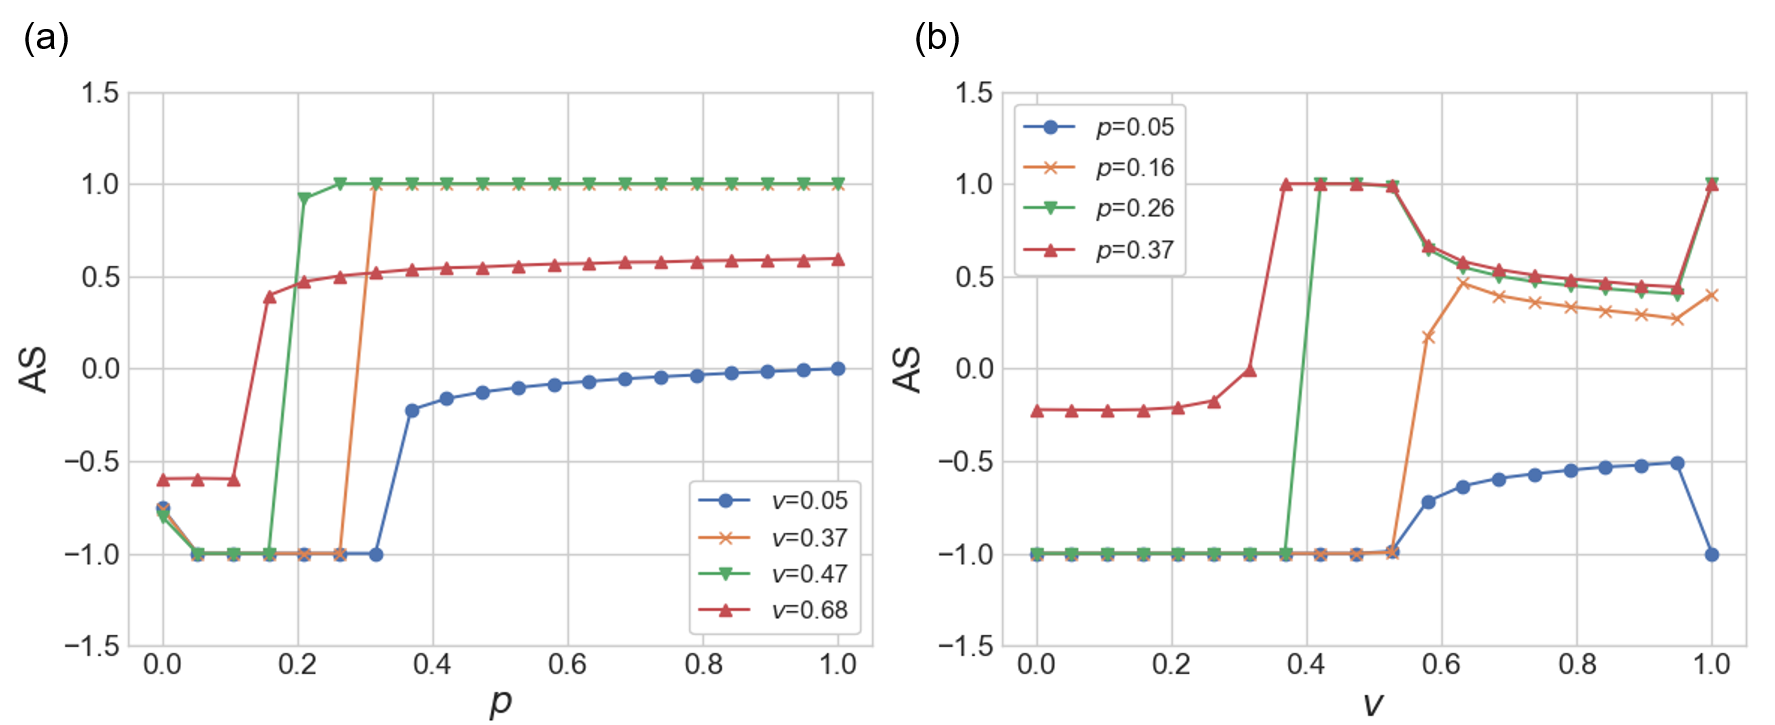
\includegraphics[width=\hsize]{AS_2d.png}
	\caption{(a) $p$-\textit{AS} chart according to certain $v$ values. (b) $v$-\textit{AS} chart according to certain $p$ values.}
	\label{AS_2d}
\end{figure*}

\begin{figure}[!htb]
	\centering
	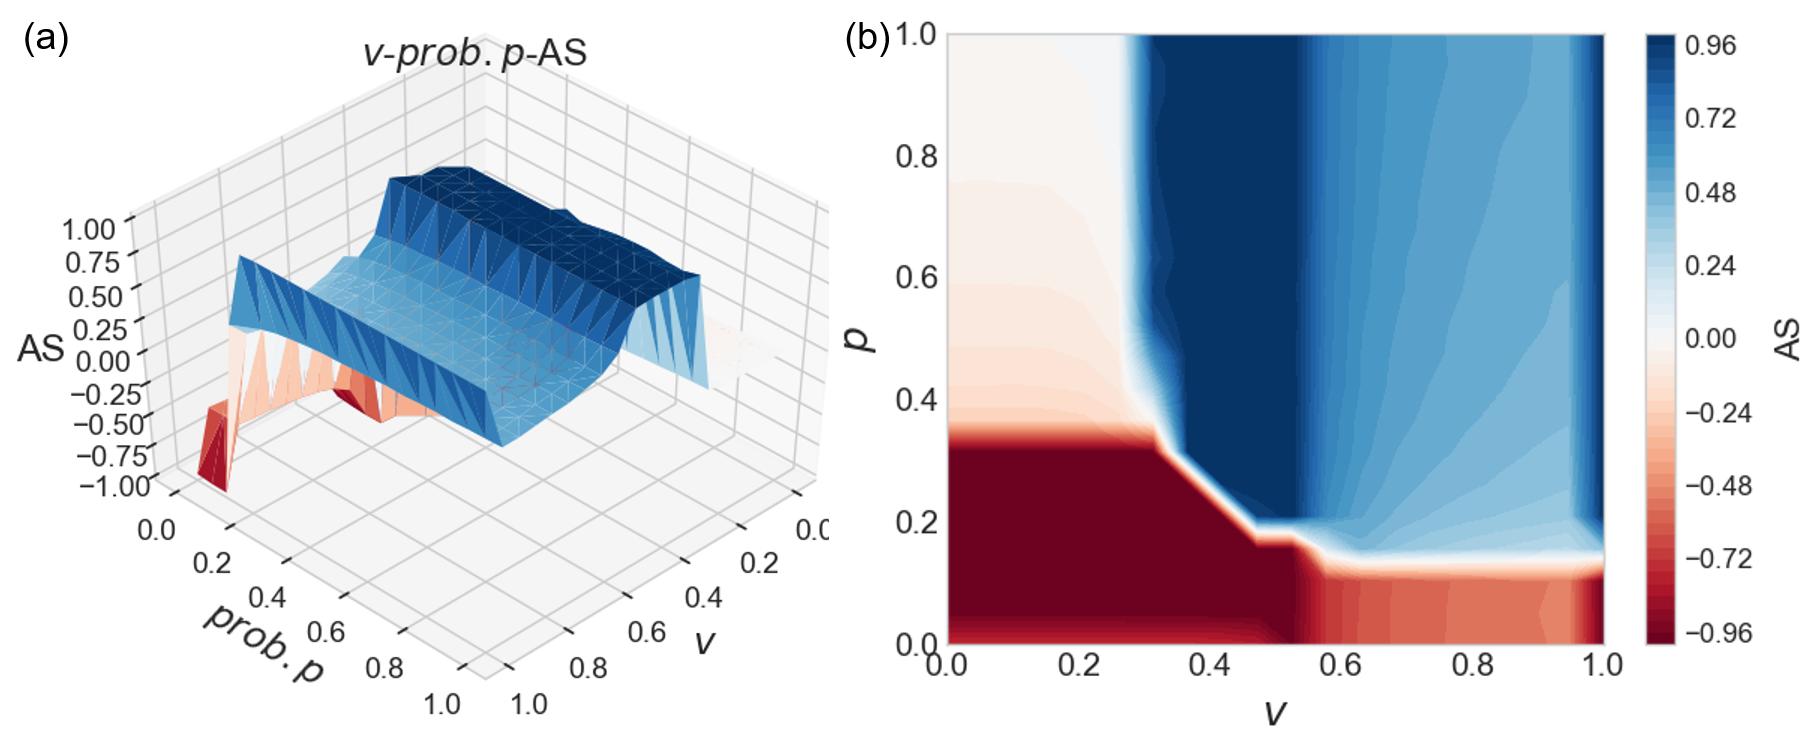
\includegraphics[width=\hsize]{p_v_AS_3d.png}
	\caption{Two layer networks with sequential updating rule : \textit{AS} changing with all $p$ and $v$}
	\label{p_v_AS_3d}
\end{figure}



\chapter{Competition on two layer with different structural network}
\label{chap:competition on two layer with different structural network}


\section{Competition on Networks with different number of external links}

In this subsection, we consider the influence of external links. Based on the basic model in Subsection 3.1, we reduce the number of nodes in layer B at a certain rate and increase the external links from nodes in layer B accordingly.  We denote \textit{HM(n)} as a hierarchical model with a level $n$, which means that the number of nodes in layer B is $1/n$ of the number of nodes in layer A, and the number of external links from node in layer B is $n$ in view that the number of external links from node in layer A is $1$. In other words, each node in layer A has one external edge, but each node in layer B has $n$ external edges for \textit{HM(n)}, which means one node in layer B can be influenced by $n$ nodes in layer A. $\gamma$ scale is same as the Random Regular Networks Model. But, $\beta$ scale depends on the number of degrees. So the $\beta$ scale is adjusted to have the same probability of volatility with Random Regular Networks Model(\textit{RRM}) as following Equation.
\begin{equation}
{\beta _{h,\max}} = {\beta _{rr,\max}} \cdot \log \left( {\frac{{{n_{rr}}^{ - {S_i}}}}{{{i_{rr,i}} + {e_{rr,i}}}} \cdot \frac{{{i_{h,i}} + {e_{h,i}}}}{{{n_{h}}^{ - {S_i}}}}} \right). 
\end{equation}

Eq(6) is derived from Eq(1) at the initial states. $\beta _{h,\max}$ is the maximum value of $\beta$ scale in \textit{HM}, and $\beta _{rr,\max}$ is the maximum value of $\beta$ scale in \textit{RRM}. When \textit{RRM} begins with initial state and the maximum of $\beta$ scale, it has the lowest volatility except $0$. In order to have the same probability in layer B dynamics for different network structures at the initial time, maximum value of $\beta$ in \textit{HM} is calculated based on Eq(6). 

Fig.~\ref{Fig4} shows the Hierarchical Model simulation results. Comparing \textit{HMs} with \textit{RRM}, \textit{CR} and \textit{PCR} are all increased remarkably. \textit{HMs} have more positive consensus part than \textit{RRM}. It shows that as the number of B nodes are decreased, it is easy to make positive consensus. Comparing \textit{HM(16)} with other \textit{HMs}, \textit{HM(16)} has the most positive consensus part. In case of models where the number of nodes in layer B is less than \textit{HM(16)},  \textit{CR} and \textit{PCR} of the models are decreased and \textit{NCR} is increased slightly. Also, for models where the number of nodes in layer B is more than \textit{HM(16)}, \textit{CR} and \textit{PCR} are also decreased. However, \textit{HM(4)} has the most \textit{AS total}. Although \textit{HM(4)} doesn't have the most consensus part, it has more intensity for positive social opinion. It can be analyzed that strong social intensity usually can not make more consensus. These results indicate that network structure can contribute more for consensus. 

\begin{figure}[!htb]
	\centering
	\includegraphics[width=\hsize]{FIG4.png}
	\caption{Hierarchical Model(\textit{HM(n)})}
	\label{Fig4}
\end{figure}

In summary, all the Hierarchical Models have more consensus ratio than Random Regular Networks Model. Among \textit{HMs}, \textit{HM(16)} has the most positive consensus part. When the number of nodes in layer B is more or less than \textit{HM(16)}, \textit{CR} and \textit{PCR} are decreased. This shows that there exists an efficient number for the decision making layer to perform positive consensus.  

\section{Competition on Networks with different number of internal links}
\begin{figure}[!htb]
	\centering
	\includegraphics[width=\hsize]{FIG5.png}
	\caption{Comparison of Networks with different internal degrees(\textit{RR(n)-RR(m)}: layer A has random regular network with $n$ internal edges, layer B has random regular network with $m$ internal edges)}
	\label{Fig5}
\end{figure}
Next, the interconnected networks are simulated with different internal degrees in order to define and evaluate the influence of internal degrees. The number of internal degrees on each node is switched to $2$ or $5$.

Fig.~\ref{Fig5} shows the simulation results with changing the number of internal edges. \textit{RR(5)-RR(2)} has the most \textit{PCR}. \textit{RR(2)-RR(5)} has the most \textit{NCR}. When the number of internal edges in layer A are more than layer B, it has more positive consensus. On the other hand, when the number of internal edges in layer B are more than layer A, it has relatively more negative consensus. These results provide that the number of edges on layer A has the tendency to keep positive state, and the number of edges on layer B has the tendency to keep negative state. The number of internal edges have the influence on consensus result and a layer with more internal edges has the tendency to maintain its own state. In case of networks with same internal edges, \textit{RR(2)-RR(2)} has more \textit{PCR} and \textit{AS total} than \textit{RR(5)-RR(5)}. It can be analyzed that \textit{RR(5)-RR(5)} is hard to make consensus, because it has more internal edges to cause inner conflict. Also, \textit{RR(2)-RR(2)} has less \textit{NCR} than \textit{RR(5)-RR(5)}. It shows that the number of internal edges in layer B is more sensitive than layer A. As Eq(1) shows, layer B dynamics can have more various and extreme probabilities when it has more degrees. For example, in case of \textit{RR(2)-RR(2)} with $\beta = 1$, the dynamics starts with $P_B=1/3$ and in case of \textit{RR(5)-RR(5)} with $\beta = 1$, the dynamics starts with $P_B=1/6$.    

\section{Competition on Networks with different structures}
So far, each layer of the interconnected network consisted of random regular networks that has the same number of edges for each node. Now, the simulation would be implemented on different network structures. 

\begin{figure}[!htb]
	\centering
	\includegraphics[width=\hsize]{FIG6.png}
	\caption{Comparison of Networks with different structures}
	\label{Fig6}
\end{figure}

Here, we use \textit{Barabasi-Albert network(BA)} structure as introduced in \cite{barabasi1999}. To evaluate the influence of network structure, 5 simulations are implemented with changing network structures. The \textit{BA} network is applied for both layers or switched on each layer. And, because layer A with \textit{BA} network structure has total $10,215$ internal edges, \textit{RR(10)-RR(5)}, under the similar conditions such as the number of nodes and edges, is also simulated. The simulation results are shown in Fig.~\ref{Fig6}. The result of \textit{BA-RR} and \textit{RR(10)-RR(5)} have almost the same features. The gap of \textit{CR} is almost same(less than 0.01). The structure of network make no obvious difference of consensus results. In case of \textit{BA-BA}, the \textit{CR} has the least ratio for consensus. \textit{BA-BA} structure has lots of internal edges on each layer. Therefore, it is hard to make consensus due to inner conflict on each layer. 





\subsection{无序列表}
\label{sec:unorderlist}

以下是一个无序列表的例子,列表的每个条目单独分段。

\begin{itemize}
  \item 这是一个无序列表。
  \item 这是一个无序列表。
  \item 这是一个无序列表。
\end{itemize}

使用\verb+itemize*+环境可以创建行内无序列表。
\begin{itemize*}
  \item 这是一个无序列表。
  \item 这是一个无序列表。
  \item 这是一个无序列表。
\end{itemize*}
行内无序列表条目不单独分段,所有内容直接插入在原文的段落中。

\subsection{有序列表}
\label{sec:orderlist}

使用环境\verb+enumerate+和\verb+enumerate*+创建有序列表,
使用方法无序列表类似。

\begin{enumerate}
  \item 这是一个有序列表。
  \item 这是一个有序列表。
  \item 这是一个有序列表。
\end{enumerate}

使用\verb+enumerate*+环境可以创建行内有序列表。
\begin{enumerate*}
  \item 这是一个默认有序列表。
  \item 这是一个默认有序列表。
  \item 这是一个默认有序列表。
\end{enumerate*}
行内有序列表条目不单独分段,所有内容直接插入在原文的段落中。

\subsection{描述型列表}

使用环境\verb+description+可创建带有主题词的列表,条目语法是\verb+\item[主题] 内容+。
\begin{description}
    \item[主题一] 详细内容
    \item[主题二] 详细内容
    \item[主题三] 详细内容 \ldots
\end{description}

\subsection{自定义列表样式}

可以使用\verb+label+参数控制列表的样式,
详细可以参考WikiBooks\footnote{\url{https://en.wikibooks.org/wiki/LaTeX/List_Structures\#Customizing_lists}}。
比如一个自定义样式的行内有序列表
\begin{enumerate*}[label=\itshape\alph*)\upshape]
  \item 这是一个自定义样式有序列表。
  \item 这是一个自定义样式有序列表。
  \item 这是一个自定义样式有序列表。
\end{enumerate*}

\section{数学排版}
\label{sec:matheq}

\subsection{公式排版}
\label{sec:eqformat}

这里有举一个长公式排版的例子,来自\href{http://www.tex.ac.uk/tex-archive/info/math/voss/mathmode/Mathmode.pdf}{《Math mode》}:

\begin {multline}
  \frac {1}{2}\Delta (f_{ij}f^{ij})=
  2\left (\sum _{i<j}\chi _{ij}(\sigma _{i}-
    \sigma _{j}) ^{2}+ f^{ij}\nabla _{j}\nabla _{i}(\Delta f)+\right .\\
  \left .+\nabla _{k}f_{ij}\nabla ^{k}f^{ij}+
    f^{ij}f^{k}\left [2\nabla _{i}R_{jk}-
      \nabla _{k}R_{ij}\right ]\vphantom {\sum _{i<j}}\right )
\end{multline}

\subsection{SI单位}

使用\verb+siunitx+宏包可以方便地输入SI单位制单位,例如\verb+\SI{5}{\um}+可以得到\SI{5}{\um}。

\subsubsection{一个四级标题}
\label{sec:depth4}

这是全文唯一的一个四级标题。在这部分中将演示了mathtools宏包中可伸长符号(箭头、等号的例子)的例子。

\begin{displaymath}
    A \xleftarrow[n=0]{} B \xrightarrow[LongLongLongLong]{n>0} C
\end{displaymath}

\begin{eqnarray}
  f(x) & \xleftrightarrow[]{A=B}  & B \\
  & \xleftharpoondown[below]{above} & B \nonumber \\
  & \xLeftrightarrow[below]{above} & B
\end{eqnarray}

又如:

\begin{align}
  \label{eq:none}
  & I(X_3;X_4)-I(X_3;X_4\mid{}X_1)-I(X_3;X_4\mid{}X_2) \nonumber \\
  = & [I(X_3;X_4)-I(X_3;X_4\mid{}X_1)]-I(X_3;X_4\mid{}\tilde{X}_2) \\
  = & I(X_1;X_3;X_4)-I(X_3;X_4\mid{}\tilde{X}_2)
\end{align}

\subsection{定理环境}

模板中定义了丰富的定理环境
algo(算法),thm(定理),lem(引理),prop(命题),cor(推论),defn(定义),conj(猜想),exmp(例),rem(注),case(情形),
bthm(断言定理),blem(断言引理),bprop(断言命题),bcor(断言推论)。
amsmath还提供了一个proof(证明)的环境。
这里举一个“定理”和“证明”的例子。
\begin{thm}[留数定理]
\label{thm:res}
  假设$U$是复平面上的一个单连通开子集,$a_1,\ldots,a_n$是复平面上有限个点,$f$是定义在$U\backslash \{a_1,\ldots,a_n\}$上的全纯函数,
  如果$\gamma$是一条把$a_1,\ldots,a_n$包围起来的可求长曲线,但不经过任何一个$a_k$,并且其起点与终点重合,那么:

  \begin{equation}
    \label{eq:res}
    \ointop_{\gamma}f(z)\,\mathrm{d}z = 2\uppi\mathbf{i}\sum^n_{k=1}\mathrm{I}(\gamma,a_k)\mathrm{Res}(f,a_k)
  \end{equation}

  如果$\gamma$是若尔当曲线,那么$\mathrm{I}(\gamma, a_k)=1$,因此:

  \begin{equation}
    \label{eq:resthm}
    \ointop_{\gamma}f(z)\,\mathrm{d}z = 2\uppi\mathbf{i}\sum^n_{k=1}\mathrm{Res}(f,a_k)
  \end{equation}

      % \oint_\gamma f(z)\, dz = 2\pi i \sum_{k=1}^n \mathrm{Res}(f, a_k ).

  在这里,$\mathrm{Res}(f, a_k)$表示$f$在点$a_k$的留数,$\mathrm{I}(\gamma,a_k)$表示$\gamma$关于点$a_k$的卷绕数。
  卷绕数是一个整数,它描述了曲线$\gamma$绕过点$a_k$的次数。如果$\gamma$依逆时针方向绕着$a_k$移动,卷绕数就是一个正数,
  如果$\gamma$根本不绕过$a_k$,卷绕数就是零。

  定理\ref{thm:res}的证明。

  \begin{proof}
    首先,由……

    其次,……

    所以……
  \end{proof}
\end{thm}

上面的公式例子中,有一些细节希望大家注意。微分号d应该使用“直立体”也就是用mathrm包围起来。
并且,微分号和被积函数之间应该有一段小间隔,可以插入\verb+\,+得到。
斜体的$d$通常只作为一般变量。
i,j作为虚数单位时,也应该使用“直立体”为了明显,还加上了粗体,例如\verb+\mathbf{i}+。斜体$i,j$通常用作表示“序号”。
其他字母在表示常量时,也推荐使用“直立体”譬如,圆周率$\uppi$(需要upgreek宏包),自然对数的底$\mathrm{e}$。
不过,我个人觉得斜体的$e$和$\pi$很潇洒,在不至于引起混淆的情况下,我也用这两个字母的斜体表示对应的常量。


\section{向文档中插入图像}
\label{sec:insertimage}

\subsection{支持的图片格式}
\label{sec:imageformat}

\XeTeX 可以很方便地插入PDF、PNG、JPG格式的图片。

插入PNG/JPG的例子如\ref{fig:SRR}所示。
这两个水平并列放置的图共享一个“图标题”(table caption),没有各自的小标题。

\begin{figure}[!htp]
  \centering
  
\includegraphics[width=4cm]{example/sjtulogo.png}
  \hspace{1cm}
  
\includegraphics[width=4cm]{example/sjtulogo.jpg}
  \bicaption[这里将出现在插图索引中]
    {中文题图}
    {English caption}
  \label{fig:SRR}
\end{figure}

这里还有插入EPS图像和PDF图像的例子,如图\ref{fig:epspdf:a}和图\ref{fig:epspdf:b}。这里将EPS和PDF图片作为子图插入,每个子图有自己的小标题。子图标题使用subcaption宏包添加。

\begin{figure}[!htp]
  \centering
  \subcaptionbox{EPS 图像\label{fig:epspdf:a}}[3cm] %标题的长度,超过则会换行,如下一个小图。
    {
\includegraphics[height=2.5cm]{example/sjtulogo.eps}}
  \hspace{4em}
  \subcaptionbox{PDF 图像,注意这个图略矮些。如果标题很长的话,它会自动换行\label{fig:epspdf:b}}
    {
\includegraphics[height=2cm]{sjtulogo.pdf}}
  \bicaption{插入eps和pdf的例子(使用 subcaptionbox 方式)}{An EPS and PDF demo with subcaptionbox}
  \label{fig:pdfeps-subcaptionbox}
\end{figure}

\begin{figure}[!htp]
  \centering
  \begin{subfigure}{2.5cm}
    \centering
    
\includegraphics[height=2.5cm]{example/sjtulogo.eps}
    \caption{EPS 图像}
  \end{subfigure}
  \hspace{4em}
  \begin{subfigure}{0.4\textwidth}
    \centering
    
\includegraphics[height=2cm]{sjtulogo.pdf}
    \caption{PDF 图像,注意这个图略矮些。subfigure中同一行的子图在顶端对齐。}
  \end{subfigure}
  \bicaption{插入eps和pdf的例子(使用 subfigure 方式)}{An EPS and PDF demo with subfigure}
  \label{fig:pdfeps-subfigure}
\end{figure}

更多关于 \LaTeX 插图的例子可以参考\href{http://www.cs.duke.edu/junhu/Graphics3.pdf}{《\LaTeX 插图指南》}。

\subsection{长标题的换行}
\label{sec:longcaption}

图\ref{fig:longcaptionbad}和图\ref{fig:longcaptiongood}都有比较长图标题,通过对比发现,图\ref{fig:longcaptiongood}的换行效果更好一些。
其中使用了minipage环境来限制整个浮动体的宽度。

\begin{figure}[!htp]
  \centering
  
\includegraphics[width=4cm]{sjtubadge.pdf}
  \bicaption[这里将出现在插图索引]
    {上海交通大学是我国历史最悠久的高等学府之一,是教育部直属、教育部与上海市共建的全国重点大学.}
    {Where there is a will, there is a way.}
 \label{fig:longcaptionbad}
\end{figure}

\begin{figure}[!htbp]
  \centering
  \begin{minipage}[b]{0.6\textwidth}
    \centering
    
\includegraphics[width=4cm]{sjtubadge.pdf}
    \bicaption[出现在插图索引中]
      {上海交通大学是我国历史最悠久的高等学府之一,是教育部直属、教育部与上海市共建的全国重点大学.}
      {Where there is a will, there is a way.}
    \label{fig:longcaptiongood}
  \end{minipage}
\end{figure}

\subsection{添加图注}

当插图中组成部件由数字或字母等编号表示时,可在插图下方添加图注进行说明,如图\ref{fig:cn_100t}所示。

\begin{figure}[!htp]
  \centering
  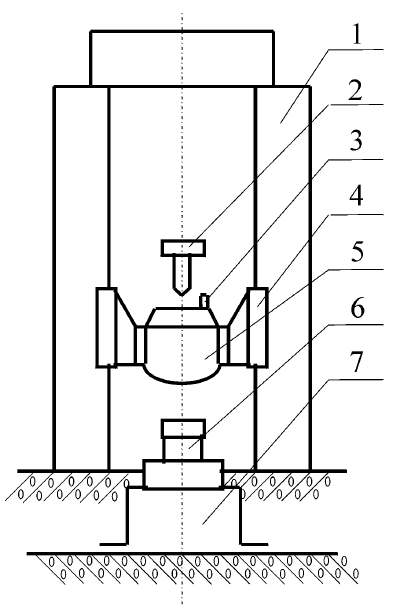
\includegraphics[width=0.3\textwidth]{example/cn_100t.png}\
  \begin{center}
    \small\kaishu 1.立柱 2.提升释放机构 3.标准冲击加速度计 \\ 4.导轨 5.重锤 6.被校力传感器 7.底座
  \end{center}
  \vspace{-1em}
  \bicaption[出现在插图索引中]
    {示例图片来源于\parencite{he1999}}
    {Stay hungry, stay foolish.}
 \label{fig:cn_100t}
\end{figure}

\subsection{绘制流程图}

图\ref{fig:flow_chart}是一张流程图示意。使用tikz环境,搭配四种预定义节点(\verb+startstop+、\verb+process+、\verb+decision+和\verb+io+),可以容易地绘制出流程图。
\begin{figure}[!htp]
    \centering
    \resizebox{6cm}{!}{\begin{tikzpicture}[node distance=2cm]
    \node (pic) [startstop] {待测图片};
    \node (bg) [io, below of=pic] {读取背景};
    \node (pair) [process, below of=bg] {匹配特征点对};
    \node (threshold) [decision, below of=pair, yshift=-0.5cm] {多于阈值};
    \node (clear) [decision, right of=threshold, xshift=3cm] {清晰?};
    \node (capture) [process, right of=pair, xshift=3cm, yshift=0.5cm] {重采};
    \node (matrix_p) [process, below of=threshold, yshift=-0.8cm] {透视变换矩阵};
    \node (matrix_a) [process, right of=matrix_p, xshift=3cm] {仿射变换矩阵};
    \node (reg) [process, below of=matrix_p] {图像修正};
    \node (return) [startstop, below of=reg] {配准结果};
     
    %连接具体形状
    \draw [arrow](pic) -- (bg);
    \draw [arrow](bg) -- (pair);
    \draw [arrow](pair) -- (threshold);

    \draw [arrow](threshold) -- node[anchor=south] {否} (clear);

    \draw [arrow](clear) -- node[anchor=west] {否} (capture);
    \draw [arrow](capture) |- (pic);
    \draw [arrow](clear) -- node[anchor=west] {是} (matrix_a);
    \draw [arrow](matrix_a) |- (reg);

    \draw [arrow](threshold) -- node[anchor=east] {是} (matrix_p);
    \draw [arrow](matrix_p) -- (reg);
    \draw [arrow](reg) -- (return);
\end{tikzpicture}
}
    \bicaption{绘制流程图效果}{Flow chart}
    \label{fig:flow_chart}
\end{figure}

\clearpage

\section{表格}
\label{sec:tab}

这一节给出的是一些表格的例子,如表\ref{tab:firstone}所示。

\begin{table}[!hpb]
  \centering
  \bicaption[指向一个表格的表目录索引]
    {一个颇为标准的三线表格\footnotemark[1]}
    {A Table}
  \label{tab:firstone}
  \begin{tabular}{@{}llr@{}} \toprule
    \multicolumn{2}{c}{Item} \\ \cmidrule(r){1-2}
    Animal & Description & Price (\$)\\ \midrule
    Gnat & per gram & 13.65 \\
    & each & 0.01 \\
    Gnu & stuffed & 92.50 \\
    Emu & stuffed & 33.33 \\
    Armadillo & frozen & 8.99 \\ \bottomrule
  \end{tabular}
\end{table}
\footnotetext[1]{这个例子来自\href{http://www.ctan.org/tex-archive/macros/latex/contrib/booktabs/booktabs.pdf}{《Publication quality tables in LATEX》}(booktabs宏包的文档)。这也是一个在表格中使用脚注的例子,请留意与threeparttable实现的效果有何不同。}

下面一个是一个更复杂的表格,用threeparttable实现带有脚注的表格,如表\ref{tab:footnote}。

\begin{table}[!htpb]
  \bicaption[出现在表目录的标题]
    {一个带有脚注的表格的例子}
    {A Table with footnotes}
  \label{tab:footnote}
  \centering
  \begin{threeparttable}[b]
     \begin{tabular}{ccd{4}cccc}
      \toprule
      \multirow{2}{6mm}{total}&\multicolumn{2}{c}{20\tnote{1}} & \multicolumn{2}{c}{40} &  \multicolumn{2}{c}{60}\\
      \cmidrule(lr){2-3}\cmidrule(lr){4-5}\cmidrule(lr){6-7}
      &www & \multicolumn{1}{c}{k} & www & k & www & k \\ % 使用说明符 d 的列会自动进入数学模式,使用 \multicolumn 对文字表头做特殊处理
      \midrule
      &$\underset{(2.12)}{4.22}$ & 120.0140\tnote{2} & 333.15 & 0.0411 & 444.99 & 0.1387 \\
      &168.6123 & 10.86 & 255.37 & 0.0353 & 376.14 & 0.1058 \\
      &6.761    & 0.007 & 235.37 & 0.0267 & 348.66 & 0.1010 \\
      \bottomrule
    \end{tabular}
    \begin{tablenotes}
    \item [1] the first note.% or \item [a]
    \item [2] the second note.% or \item [b]
    \end{tablenotes}
  \end{threeparttable}
\end{table}

\section{参考文献管理}

 \LaTeX 具有将参考文献内容和表现形式分开管理的能力,涉及三个要素:参考文献数据库、参考文献引用格式、在正文中引用参考文献。
这样的流程需要多次编译:

\begin{enumerate}[noitemsep,topsep=0pt,parsep=0pt,partopsep=0pt]
	\item 用户将论文中需要引用的参考文献条目,录入纯文本数据库文件(bib文件)。
	\item 调用xelatex对论文模板做第一次编译,扫描文中引用的参考文献,生成参考文献入口文件(aux)文件。
	\item 调用bibtex,以参考文献格式和入口文件为输入,生成格式化以后的参考文献条目文件(bib)。
	\item 再次调用xelatex编译模板,将格式化以后的参考文献条目插入正文。
\end{enumerate}

参考文献数据库(thesis.bib)的条目,可以从Google Scholar搜索引擎\footnote{\url{https://scholar.google.com}}、CiteSeerX搜索引擎\footnote{\url{http://citeseerx.ist.psu.edu}}中查找,文献管理软件Papers\footnote{\url{http://papersapp.com}}、Mendeley\footnote{\url{http://www.mendeley.com}}、JabRef\footnote{\url{http://jabref.sourceforge.net}}也能够输出条目信息。

下面是在Google Scholar上搜索到的一条文献信息,格式是纯文本:

\begin{lstlisting}[caption={从Google Scholar找到的参考文献条目}, label=googlescholar, escapeinside="", numbers=none]
    @phdthesis{"白2008信用风险传染模型和信用衍生品的定价",
      title={"信用风险传染模型和信用衍生品的定价"},
      author={"白云芬"},
      year={2008},
      school={"上海交通大学"}
    }
\end{lstlisting}

推荐修改后在bib文件中的内容为:

\begin{lstlisting}[caption={修改后的参考文献条目}, label=itemok, escapeinside="", numbers=none]
  @phdthesis{bai2008,
    title={"信用风险传染模型和信用衍生品的定价"},
    author={"白云芬"},
    date={2008},
    address={"上海"},
    school={"上海交通大学"}
  }
\end{lstlisting}

按照教务处的要求,参考文献外观应符合国标GBT7714的要求\footnote{\url{http://www.cces.net.cn/guild/sites/tmxb/Files/19798_2.pdf}}。
在模板中,表现形式的控制逻辑通过biblatex-gb7714-2015包实现\footnote{\url{https://www.ctan.org/pkg/biblatex-gb7714-2015}},基于{Bib\LaTeX}管理文献。在目前的多数TeX发行版中,可能都没有默认包含biblatex-gb7714-2015,需要手动安装。

正文中引用参考文献时,用\verb+\cite{key1,key2,key3...}+可以产生“上标引用的参考文献”,
如\cite{Meta_CN,chen2007act,DPMG}。
使用\verb+\parencite{key1,key2,key3...}+则可以产生水平引用的参考文献,例如\parencite{JohnD,zhubajie,IEEE-1363}。
请看下面的例子,将会穿插使用水平的和上标的参考文献:关于书的\parencite{Meta_CN,JohnD,IEEE-1363},关于期刊的\cite{chen2007act,chen2007ewi},
会议论文\parencite{DPMG,kocher99,cnproceed},
硕士学位论文\parencite{zhubajie,metamori2004},博士学位论文\cite{shaheshang,FistSystem01,bai2008},标准文件\parencite{IEEE-1363},技术报告\cite{NPB2},电子文献\parencite{xiaoyu2001, CHRISTINE1998},用户手册\parencite{RManual}。

总结一些注意事项:
\begin{itemize}
\item 参考文献只有在正文中被引用了,才会在最后的参考文献列表中出现;
\item 参考文献“数据库文件”bib是纯文本文件,请使用UTF-8编码,不要使用GBK编码;
\item 参考文献条目中默认通过date域输入时间。兼容使用year域时会产生编译warning,可忽略。
\end{itemize}

\section{用listings插入源代码}

原先ctexbook文档类和listings宏包配合使用时,代码在换页时会出现莫名其妙的错误,后来经高人指点,顺利解决了。
感兴趣的话,可以看看\href{http://bbs.ctex.org/viewthread.php?tid=53451}{这里}。
这里给使用listings宏包插入源代码的例子,这里是一段C代码。
另外,listings宏包真可谓博大精深,可以实现各种复杂、漂亮的效果,想要进一步学习的同学,可以参考
\href{http://mirror.ctan.org/macros/latex/contrib/listings/listings.pdf}{listings宏包手册}。

\begin{lstlisting}[language={C}, caption={一段C源代码}]
#include <stdio.h>
#include <unistd.h>
#include <sys/types.h>
#include <sys/wait.h>

int main() {
  pid_t pid;

  switch ((pid = fork())) {
  case -1:
    printf("fork failed\n");
    break;
  case 0:
    /* child calls exec */
    execl("/bin/ls", "ls", "-l", (char*)0);
    printf("execl failed\n");
    break;
  default:
    /* parent uses wait to suspend execution until child finishes */
    wait((int*)0);
    printf("is completed\n");
    break;
  }

  return 0;
}
\end{lstlisting}

\section{用algorithm和algorithmicx宏包插入算法描述}

algorithmicx 比 algorithmic 增加了一些命令。
示例如算法\ref{algo:sum_100}和算法\ref{algo:merge_sort},
后者的代码来自\href{http://hustsxh.is-programmer.com/posts/38801.html}{xhSong的博客}。
algorithmicx的详细使用方法见\href{http://mirror.hust.edu.cn/CTAN/macros/latex/contrib/algorithmicx/algorithmicx.pdf}{官方README}。
使用算法宏包时,算法出现的位置很多时候不按照tex文件里的书写顺序,
需要强制定位时可以使用\verb+\begin{algorithm}[H]+
\footnote{http://tex.stackexchange.com/questions/165021/fixing-the-location-of-the-appearance-in-algorithmicx-environment}

这是写在算法\ref{algo:sum_100}前面的一段话,在生成的文件里它会出现在算法\ref{algo:sum_100}前面。

\begin{algorithm}
% \begin{algorithm}[H] % 强制定位
\caption{求100以内的整数和}
\label{algo:sum_100}
\begin{algorithmic}[1] %每行显示行号
\Ensure 100以内的整数和 % 输出
\State $sum \gets 0$
\For{$i = 0 \to 100$}
    \State $sum \gets sum + i$
  \EndFor
\end{algorithmic}
\end{algorithm}

这是写在两个算法中间的一段话,当算法\ref{algo:sum_100}不使用\verb+\begin{algorithm}[H]+时它也会出现在算法\ref{algo:sum_100}前面。

对于很长的算法,单一的算法块\verb+\begin{algorithm}...\end{algorithm}+是不能自动跨页的
\footnote{http://tex.stackexchange.com/questions/70733/latex-algorithm-not-display-under-correct-section},
会出现的情况有:

\begin{itemize}
  \item 该页放不下当前的算法,留下大片空白,算法在下一页显示
  \item 单一页面放不下当前的算法,显示时超过页码的位置直到超出整个页面范围
\end{itemize}

解决方法有:

\begin{itemize}
  \item (推荐)使用\verb+algstore{algname}+和\verb+algrestore{algname}+来讲算法分为两个部分\footnote{http://tex.stackexchange.com/questions/29816/algorithm-over-2-pages},如算法\ref{algo:merge_sort}。
  \item 人工拆分算法为多个小的部分。
\end{itemize}

\begin{algorithm}
% \begin{algorithm}[H] % 强制定位
\caption{用归并排序求逆序数}
\label{algo:merge_sort}
\begin{algorithmic}[1] %每行显示行号
\Require $Array$数组,$n$数组大小 % 输入
\Ensure 逆序数 % 输出
\Function {MergerSort}{$Array, left, right$}
  \State $result \gets 0$
  \If {$left < right$}
    \State $middle \gets (left + right) / 2$
    \State $result \gets result +$ \Call{MergerSort}{$Array, left, middle$}
    \State $result \gets result +$ \Call{MergerSort}{$Array, middle, right$}
    \State $result \gets result +$ \Call{Merger}{$Array,left,middle,right$}
  \EndIf
  \State \Return{$result$}
\EndFunction
\State %空一行
\Function{Merger}{$Array, left, middle, right$}
  \State $i\gets left$
  \State $j\gets middle$
  \State $k\gets 0$
  \State $result \gets 0$
  \While{$i<middle$ \textbf{and} $j<right$}
    \If{$Array[i]<Array[j]$}
      \State $B[k++]\gets Array[i++]$
    \Else
      \State $B[k++] \gets Array[j++]$
      \State $result \gets result + (middle - i)$
    \EndIf
  \EndWhile
  \algstore{MergeSort}
\end{algorithmic}
\end{algorithm}

\begin{algorithm}
\begin{algorithmic}[1]
  \algrestore{MergeSort}
  \While{$i<middle$}
    \State $B[k++] \gets Array[i++]$
  \EndWhile
  \While{$j<right$}
    \State $B[k++] \gets Array[j++]$
  \EndWhile
  \For{$i = 0 \to k-1$}
    \State $Array[left + i] \gets B[i]$
  \EndFor
  \State \Return{$result$}
\EndFunction
\end{algorithmic}
\end{algorithm}

这是写在算法\ref{algo:merge_sort}后面的一段话,
但是当算法\ref{algo:merge_sort}不使用\verb+\begin{algorithm}[H]+时它会出现在算法\ref{algo:merge_sort}
甚至算法\ref{algo:sum_100}前面。

对于算法的索引要注意\verb+\caption+和\verb+\label+的位置,
必须是先\verb+\caption+再\verb+\label+\footnote{http://tex.stackexchange.com/questions/65993/algorithm-numbering},
否则会出现\verb+\ref{algo:sum_100}+生成的编号跟对应算法上显示不一致的问题。

根据Werner的回答\footnote{http://tex.stackexchange.com/questions/53357/switch-cases-in-algorithmic}
增加了\verb+Switch+和\verb+Case+的支持,见算法\ref{algo:switch_example}。

\begin{algorithm}
\caption{Switch示例}
\label{algo:switch_example}
\begin{algorithmic}[1]
  \Switch{$s$}
    \Case{$a$}
      \Assert{0}
    \EndCase
    \Case{$b$}
      \Assert{1}
    \EndCase
    \Default
      \Assert{2}
    \EndDefault
  \EndSwitch
\end{algorithmic}
\end{algorithm}
